\section{Lernziel R1: Grundlagen der Relationalen Algebra verstehen}

\subsection{Der Student versteht den Begriff Relation und kann damit umgehen}
Eine binäre Relation \(R\) von einer Menge \(A\) nach einer Menge \(B\) ist eine Teilmenge des Kreuzproduktes \(A \times B\).
\begin{equation*}
    R \subset A \times B
\end{equation*}
Elemente aus den Mengen \(A\) und \(B\) sind also Teil der Relation \(R\). Diese Elemente werden \emph{Tupel} genannt.
\begin{equation*}
  (a,b)\in R
\end{equation*}

\subsection{Der Student kann die Elemente einer binären oder n-stelligen Relation aufzählen}
Eine \(n\)-stellige Relation \(R\) analog zur binären Relation eine Teilmenge des kartesischen Produkts. Jetzt halt nicht nur von 2, sondern von \(n\) Mengen \(A_{1}, \dotsc, A_{n}\).


\( R \subseteq A_{1} \times \dotsb \times A_{n}\)mit \(A_1 \times \dotsb \times A_n = \{(a_1, \dotsc, a_n) \mid a_1 \in A_1, \dotsc, a_n \in A_n\}\).

\subsection{Der Student versteht den Unterschied zwischen Relationen und Funktionen}
Relationen sind allgemeinere Funktionen. Die Abbildung \ref{eq:relation-definition} erklärt den Unterschied anhand von zwei Zahlenmengen.

\begin{figure}[h!]
	\centering
	\begin{subfigure}[b]{0.27\textwidth}
		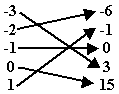
\includegraphics[width=\textwidth]{fig/funktion.png}
		\caption{Beispiel für eine Funktion}
	\end{subfigure}
	\begin{subfigure}[b]{0.3\textwidth}
		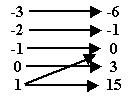
\includegraphics[width=\textwidth]{fig/relation.png}
		\caption{Beispiel für eine Relation}
	\end{subfigure}
	\caption{Relation vs. Funktion}
	\label{fig:relation-funktion}
\end{figure} 

\subsection{Der Student kann Relationen als Graphen darstellen}

\subsubsection{Graph}
Wenn die Menge beider Teile der Funktionen dieselbe ist, kann man jedes Element der Menge als Knoten und die Kanten zwischen den Knoten stellen die Relationen zwischen denen Elementen dar. Siehe Abbildung \ref{fig:relation-knoten-kanten}.

\subsubsection{Koordinatensystem}
Die einzelnen Relationen können allerdings auch als Punkte in einem Koordinatensystem eingetragen werden. Dann können auch die Relationsmengen unterschiedlich sein. Siehe Abbildung \ref{fig:relation-koordinatensystem}.

\begin{figure}[h!]
	\centering
	\begin{subfigure}[b]{0.27\textwidth}
		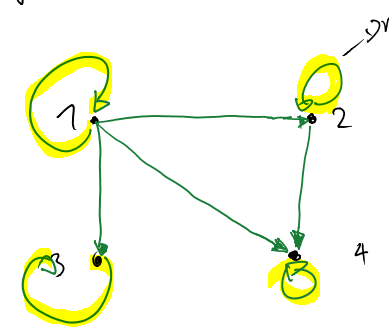
\includegraphics[width=\textwidth]{fig/knoten_kanten.png}
		\caption{Graph}
		\label{fig:relation-knoten-kanten}
	\end{subfigure}
	\begin{subfigure}[b]{0.3\textwidth}
		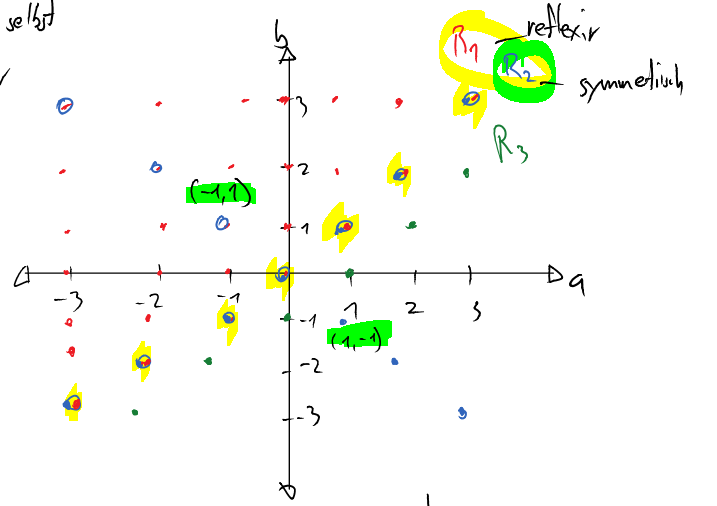
\includegraphics[width=\textwidth]{fig/koordinatensystem.png}
		\caption{Koordinatensystem}
		\label{fig:relation-koordinatensystem}
	\end{subfigure}
	\caption{Relation darstellen}
	\label{fig:relation-darstellen}
\end{figure} 

\subsection{Der Student kann reflexive, symmetrische und transitive Relationen identifizieren}

\subsubsection{Reflexive Relationen}
Bei reflexiven Relationen gilt, dass jedes Element der Menge eine Beziehung mit sich selber hat. Abbildung \ref{fig:relation-knoten-kanten} zeigt eine solche reflexive Relation (gelb markiert).

\subsubsection{Symmetrische Relation}
Eine Symmetrische Relation besagt, dass zu jeder Relation eine Relation in der Gegenrichtung da ist. Also z.B. wenn es eine Relation (1,2) gibt, muss es auch eine Relation (2,1) geben. Die Formel dazu:

\begin{equation*}
    \forall x,y \in A ((x,y) \in R \to (y,x) \in R)
\end{equation*}

\subsubsection{Transitive Relation}
Eine Relation ist transitiv, wenn es z.B. eine Relation (1,2) und eine Relation (2,3) gibt, dann muss es auch (1,3) geben. Abbildung \ref{fig:relation-knoten-kanten} zeigt eine solche transitive Relation. Formal ausgedrückt:

\begin{equation*}
  \forall x,y,z \in A ((x,y) \in R \wedge (y,z) \in R \to (x,z) \in R)
\end{equation*}


\subsection{Der Student kann überprüfen, ob eine Relation eine Äquivalenzrelation ist}
Eine Relation ist eine \emph{Äquivalenzrelation} wenn sie reflexiv, symmetrisch und transitiv ist.

\subsection{Der Student kann eine Menge, auf der eine Äquivalenzrelation definiert ist, in Äquivalenzklassen aufteilen}

Die Äquivalenzklassen der Menge $A=\{1, 2, 3, 4, 5, 6\}$ könnten beispielsweise so aussehen: $A_1=\{1, 2, 3\}, A_2=\{4, 5\}, A_3=\{6\}$. Alle Teilmengen ergeben zusammen die Menge $A$, sind nicht leer und sind paarweise disjunkt (kein Element kommt zweimal vor). 

\subsection{Der Student versteht die Korrespondenz zwischen Relationen und Tabellen}

Bei Relationen ist die Reihenfolge der Tupel wichtig. Bei Tabellen wird jedem Element des Tupels noch ein eindeutiger Name zugewiesen, weswegen dann die Reihenfolge keine Rolle mehr spielt.